\documentclass[tikz,border=5pt]{standalone}
\usepackage{tikz}
\usetikzlibrary{shapes.geometric, arrows.meta, positioning, fit, backgrounds}

\begin{document}
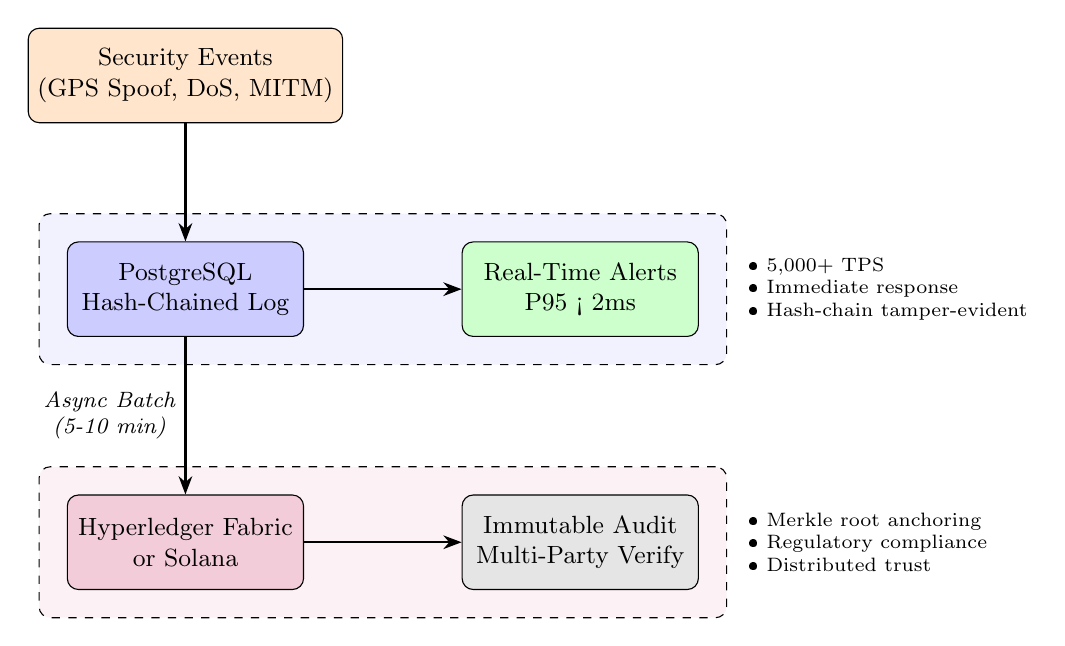
\begin{tikzpicture}[
    node distance=1.5cm,
    box/.style={
        rectangle,
        draw,
        rounded corners,
        minimum width=3cm,
        minimum height=1.2cm,
        align=center,
        font=\small
    },
    layer/.style={
        rectangle,
        draw,
        dashed,
        rounded corners,
        inner sep=10pt
    },
    arrow/.style={
        ->,
        >=Stealth,
        thick
    },
    label/.style={
        font=\footnotesize\itshape,
        align=center
    }
]

% Security Events source
\node[box, fill=orange!20] (events) {Security Events\\(GPS Spoof, DoS, MITM)};

% Real-time layer
\node[box, fill=blue!20, below=of events] (postgres) {PostgreSQL\\Hash-Chained Log};
\node[box, fill=green!20, right=2cm of postgres] (alerts) {Real-Time Alerts\\P95 < 2ms};

% Audit layer
\node[box, fill=purple!20, below=2cm of postgres] (hyperledger) {Hyperledger Fabric\\or Solana};
\node[box, fill=gray!20, right=2cm of hyperledger] (audit) {Immutable Audit\\Multi-Party Verify};

% Arrows
\draw[arrow] (events) -- (postgres);
\draw[arrow] (postgres) -- (alerts);
\draw[arrow] (postgres) -- node[left, label] {Async Batch\\(5-10 min)} (hyperledger);
\draw[arrow] (hyperledger) -- (audit);

% Layer labels
\begin{scope}[on background layer]
    \node[layer, fill=blue!5, fit=(postgres)(alerts), label={[anchor=north west]north west:\textbf{Real-Time Layer}}] {};
    \node[layer, fill=purple!5, fit=(hyperledger)(audit), label={[anchor=north west]north west:\textbf{Audit Layer}}] {};
\end{scope}

% Performance annotations
\node[right=0.5cm of alerts, font=\scriptsize, align=left] {
    \textbullet\ 5,000+ TPS\\
    \textbullet\ Immediate response\\
    \textbullet\ Hash-chain tamper-evident
};

\node[right=0.5cm of audit, font=\scriptsize, align=left] {
    \textbullet\ Merkle root anchoring\\
    \textbullet\ Regulatory compliance\\
    \textbullet\ Distributed trust
};

\end{tikzpicture}
\end{document}
